\newpage

Il existe encore de nombreuses difficultés pour expliquer les mécanismes moléculaires responsables de l’évolution de l’expression des gènes. Comme je l’ai précédemment mentionné, l'expression des gènes codant pour des protéines évolue lentement chez les vertébrés \citep{brawand_evolution_2011, necsulea_evolutionary_2014, cardoso-moreira_gene_2019}. Au contraire, les éléments \acrshort{cis}-régulateurs évoluent plus rapidement, que ce soit au niveau de leurs séquences mais aussi de leurs activités \citep{cheng_principles_2014, villar_enhancer_2015}. Peu d’études ont relié ces deux observations, et celles-ci ont révélé une faible corrélation entre le taux d’évolution de la régulation et le taux d’évolution de l’expression des gènes \citep{wong_interplay_2017, berthelot_complexity_2018}. Une hypothèse avancée met en avant la complexité et la redondance fonctionnelle des paysages \acrshort{cis}-régulateurs qui pourrait assurer une stabilité de l’expression au cours de l’évolution \citep{osterwalder_enhancer_2018, berthelot_complexity_2018}. Cependant, une autre possibilité pourrait résider dans la difficulté d’associer les éléments \acrshort{cis}-régulateurs à leurs gènes cibles. Les prédictions par une approche de voisinage des paires gènes-amplificateurs employée dans ces études pourraient en effet résulter en des associations partiellement erronées et ainsi affecter négativement les tentatives de corrélation entre leurs taux d’évolution. Les mesures expérimentales des paysages \acrshort{cis}-régulateurs par les contacts de la chromatine centrés sur les promoteurs des gènes (PCHi-C) pourraient être en mesure de fournir des associations régulatrices plus pertinentes. De telles données s’accumulent aujourd’hui sur des échantillons humains mais également sur la souris, permettant d’effectuer une analyse comparative de ces paysages \acrshort{cis}-régulateurs.\\

Ce chapitre contient le travail publié dans Genome Research au cours duquel je me suis intéressé à analyser conjointement l’évolution des paysages \acrshort{cis}-régulateurs mesurés par PCHi-C ainsi que l’évolution de l’expression des gènes. Dans un premier temps, j’ai compilé et homogénéisé l’ensemble des données de PCHi-C disponibles à l’échelle génomique pour l’humain et la souris. J’ai également réuni plusieurs prédictions d’amplificateurs obtenus à partir de différentes méthodes. Ensuite je me suis attaché à décrire plusieurs aspects de l’évolution de ces paysages \acrshort{cis}-régulateurs. J’ai d’abord analysé la conservation des séquences des régions et des amplificateurs contactés par les promoteurs des gènes au sein des génomes de 8 espèces de vertébrés (humain, souris, lapin, chien, éléphant, vache, opossum, poulet). J’ai mesuré la proportion de ces paires gènes-amplificateurs homologues conservées en synténie chez ces mêmes espèces. Entre l’humain et la souris, j’ai évalué la conservation des contacts de chromatine entre les gènes orthologues et les régions contactées homologues avec une attention particulière pour les mesures effectuées sur des types cellulaires similaires. J’ai alors utilisé des données d’expression des gènes au sein de plusieurs types cellulaires et stades de développement pour évaluer les relations entre l’évolution des paysages \acrshort{cis}-régulateur et l’évolution de l’expression des gènes chez l’humain et la souris.

\chapter{Article 2 - Long-range promoter-enhancer contacts are conserved during evolution and contribute to gene expression robustness}
\label{chap:chap3}
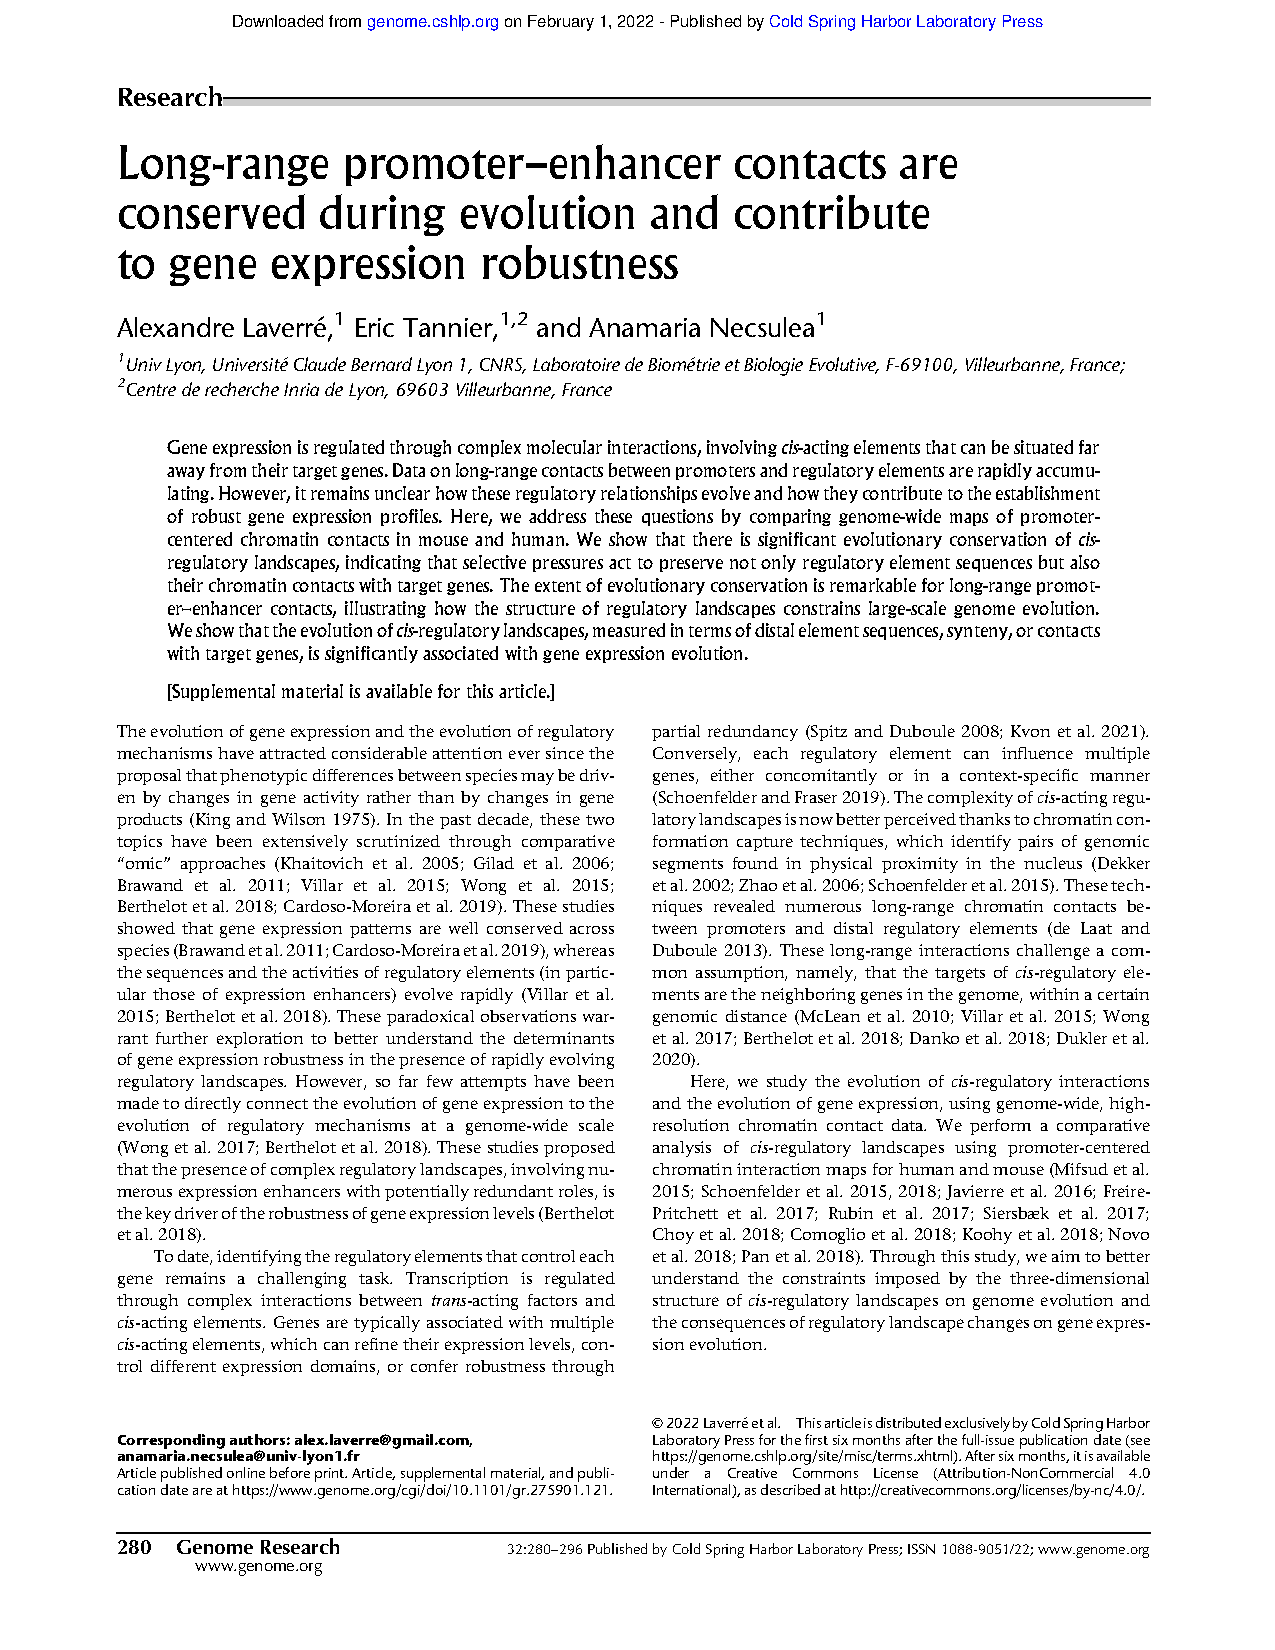
\includepdf[pages=-]{parts/11_Laverre2022.pdf}